\documentclass[a4paper]{article}
\usepackage[utf8]{inputenc}
\usepackage[russian]{babel}
\usepackage[margin=1in]{geometry}
\usepackage[sort&compress,numbers]{natbib}
\usepackage{graphicx}
\usepackage{amssymb}
\usepackage{amsmath}


\title{ДЗ1. Вероятностные распределения}
\author{Игорь Семенов, СКБ172}




\begin{document}

\maketitle



\section{Распределения и описание их основных характеристик}

\subsection{Биномиальное распределение $B(n,p)$ }
\subsubsection{Закон распределения}
$$P(\xi=k)=(\frac{n}{k})p^{k}q^{n-k},\quad k\in\{1,2,\ldots,n\}.$$

\begin{figure}[h!]
    \centering
    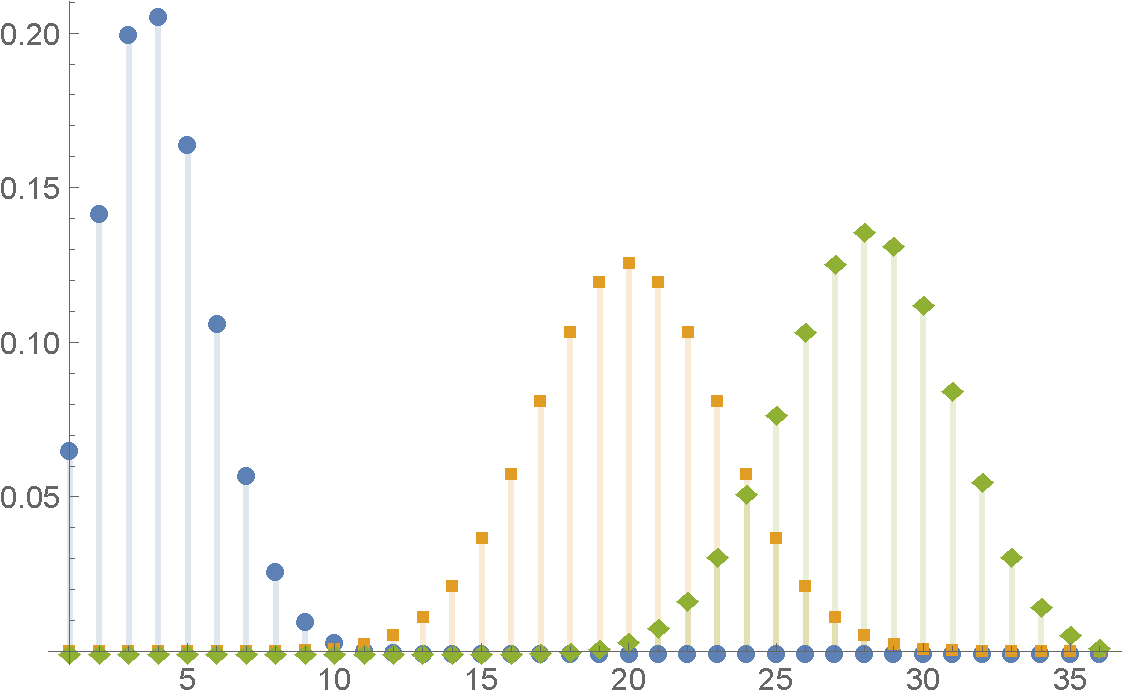
\includegraphics[scale=0.5]{BinomPDF.pdf}
    \caption{Закон распределения для $p=0.1,\,0.5,\,0.7$ при $n=40$
}
\end{figure}


\subsubsection{Математическое ожидание}
Математическое ожидание неотрицательной дискретной случайной величины называется:
$$E\xi = \sum_{i}a_ip_i=\sum_{i}a_iP(\xi=a_i)$$ Выведем математическое ожидание для Биномиального распределения:

\begin{equation*}
	\begin{split}
	E\xi   &= \sum_{k=1}^{n}k\cdot P(\xi=k)=\\
				&=\sum_{k=1}^{n}k(\frac{n}{k})p^{k}q^{n-k}=\\
				&=\sum_{k=1}^{n}k\frac{n!}{(n-k)!k!}p^{k}(1-p)^{n-k}=\\
				&=np\sum_{k=1}^{n}\frac{(n-1)!}{((n-1)-(k-1))!(k-1)!}p^{k-1}(1-p)^{(n-1)-(k-1)}=\\
                &=np(p+(1-p))^{n-1}=\\
                &=np
	\end{split}
\end{equation*}


\subsubsection{Дисперсия}
$$D\xi = E(\xi - E\xi)^2 = E\xi^2 - E^2\xi.$$
$$E\xi_i=p,\quad E{\xi_i}^2=p,\quad D\xi_i=p-p^2=p(1-p),\quad i\in {1,\ldots ,n}$$
$$D\xi = D\xi_1+D\xi_2+\ldots+D\xi_n=n p(p-1)$$

\subsubsection{Функция распределения}
$$F_\xi(x)= P(\xi<x)=\sum_{k=0}^{x}(\frac{n}{k})p^{k}q^{n-k},\quad x\in R$$
\begin{figure}[h!]
    \centering
    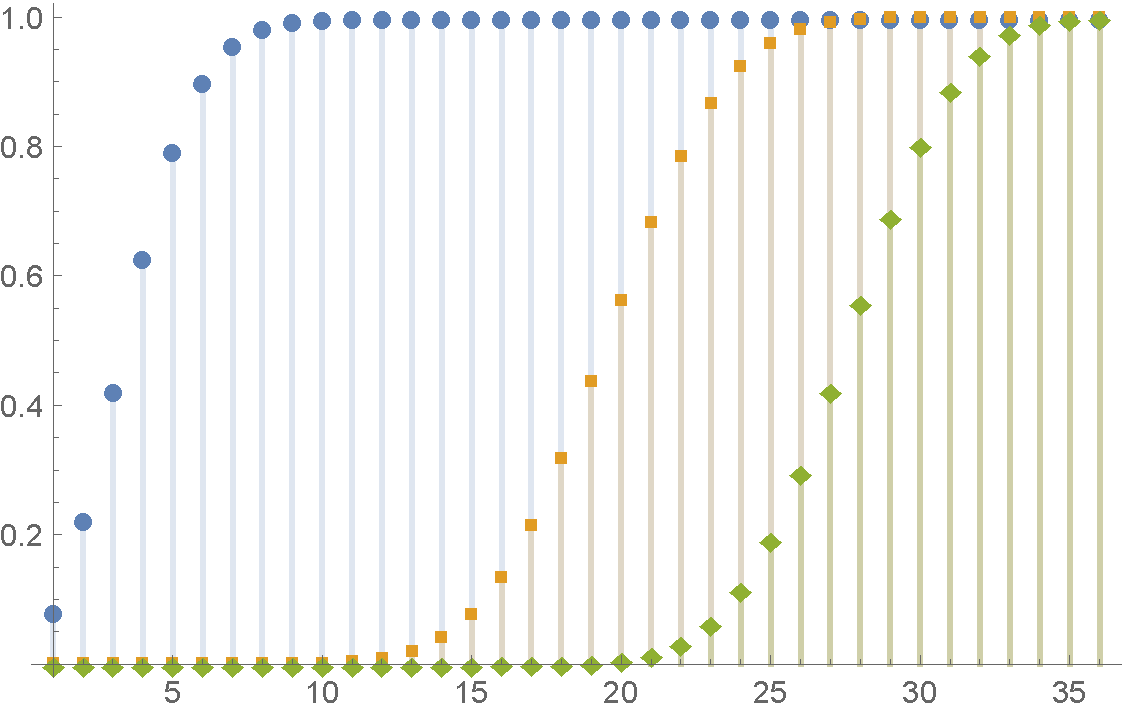
\includegraphics[scale=0.5]{BinomCDF.pdf}
    \caption{Функция распределения для $p=0.1,\,0.5,\,0.7$ при $n=40$}
\end{figure}

\subsubsection{Производящая функция}
$$\varphi(z) = \sum_{k=0}^{n}z^k p_n$$

\subsubsection{Характеристическая функция}
$$g(t) = 1-p+pe^{it}$$


\subsection{Нормальное распределение $N(\mu,\sigma^2)$}


\subsubsection{Плотность распределения}
$$f(x) = \frac{1}{\sigma\sqrt{2\pi}}e^{-\frac{(x-\mu)^2}{2{\sigma}^2}},\quad x\in R$$



\subsubsection{Функция распределения}
$$F(x) = P(\xi\leq x) = \int\limits_{-\infty}^x f(x) dx  =\bigg\vert\, x=\sigma t+\mu\,\bigg\vert = \frac{1}{\sqrt{2\pi}}\int\limits_{-\infty}^{x} e^{-\frac{t^2}{2}} dt  $$


\subsubsection{Математическое ожидание и Дисперсия}

$\xi\in N(\mu,\sigma^2)$, тогда  $\eta=(\xi-\mu)/\sigma\in N(0,1)$, где $E\eta=0$ и $D\eta=1$


Из св-ва Математического ожидания: $$E\xi = E(\sigma\eta+\mu)=\sigma E\eta + \mu = \mu$$

Из св-ва Дисперсии: $$D\xi = D(\sigma\eta+\mu)=\sigma^2 D\eta  = \sigma^2$$



\subsubsection{Производящая и характеристическая функции}
$$\varphi(z) = exp(\mu z+\frac{\sigma^2 z^2}{2}) $$
$$g(t) = exp(i\mu t+\frac{\sigma^2 t^2}{2}).$$
\begin{figure}[h!]
    \centering
    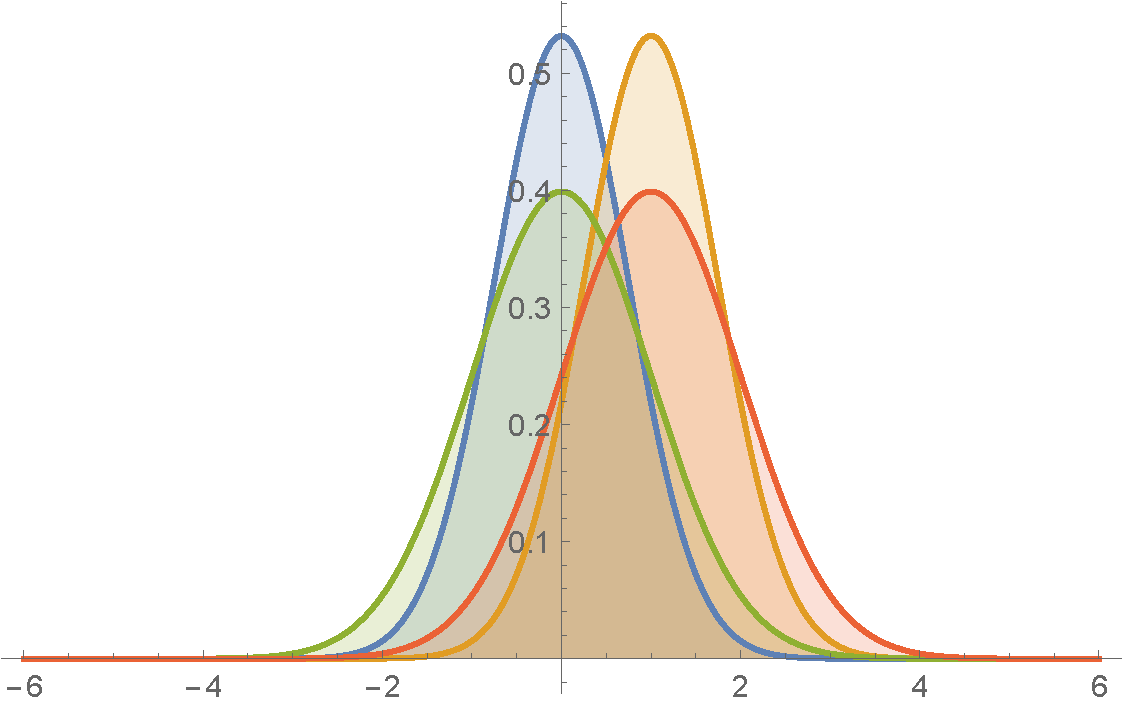
\includegraphics[scale=0.5]{NormalPDF.pdf}
    \caption{Плотности распределения для 	$\mu=0;\quad\sigma=0.75$ --- синий,\quad
	$\mu=1;\quad \sigma=0.75$ --- желтый,\quad
	$\mu=0;\quad \sigma=1$ --- зеленый,\quad
	$\mu=1;\quad \sigma=1$ --- красный
}
\end{figure}


\begin{figure}[h!]
    \centering
    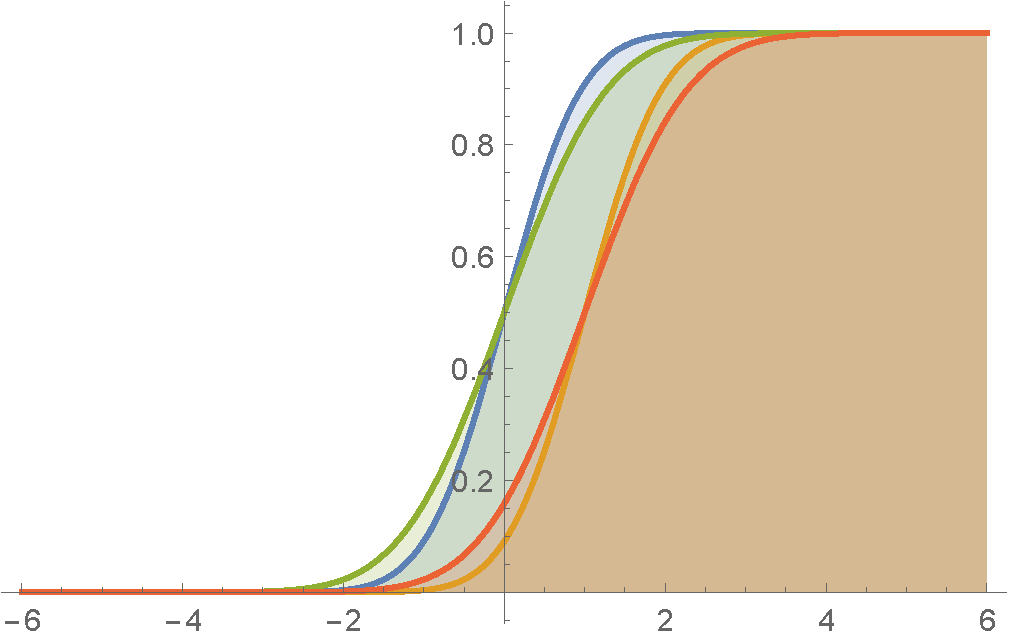
\includegraphics[scale=0.5]{NormalCDF.pdf}
    \caption{Функции распределения для 	$\mu=0;\quad\sigma=0.75$ --- синий,\quad
	$\mu=1;\quad \sigma=0.75$ --- желтый,\quad
	$\mu=0;\quad \sigma=1$ --- зеленый,\quad
	$\mu=1;\quad \sigma=1$ --- красный
}
\end{figure}


\section{Поиск примеров событий}

\subsection{Биномиальное распределение}

\subsubsection{Типичная интерпретация}
Биномиальное распределение определяет количество «успехов» в последовательности из $n$ независимых случайных экспериментов, таких, что вероятность «успеха» в каждом из них постоянна и равна $p$.

Самый распространненый пример использования биномиального распредления --- это подсчет количества выпадения орлов у монетки за $n$ бросков.

Пусть вероятность выпадения орла постоянна и равна 0.3 --- $p=0.3$, посчитаем вероятность выпадения 5 орлов за 6 бросков:
$$P(\xi=5)=\left(\begin{array}{l}{6} \\ {5}\end{array}\right)(0.3)^{5}(0.7)=0,010206$$

\subsubsection{Нетипичная интерпретация}

С помощью биномиального распределения можно считать не только успех броска монетки. Представим что мы хотим улучшить доходность нашего колл центра, где сотрудники за счет звонков продают наш товар\citep{callcenter}\\ \\
Нам известна следующая информация:

\begin{itemize}
  \item В среднем один работник делает 50 звонков в день
  \item Вероятность успешного звонка 4\%
  \item Доход с одного успешного звонка 100 \$
  \item В нашем колл центре работает 100 работников
  \item Каждый из них получает 200\$ в день
\end{itemize}

Создадим симуляцию одного дня нашего колл центра в Python

\begin{verbatim}
        # Симуляция КоллЦентра
    import numpy as np
    import matplotlib.pyplot as plt 
        # Количество работников в центре
    employees = 100
        # Зарплата работника
    wage = 200
        # Количество звонков от одного работника
    n = 50
        # Вероятность успеха каждого звонка
    p = 0.04
        # Доход за звонок
    revenue = 100
        # Биномиаальные случайные величины каждого сотрудника
    conversions = np.random.binomial(n, p, size=employees)
    
    print('Среднее значение случайной величины: ' + str(round(np.mean(conversions), 2)))
    print('Стандартное отклонение: ' + str(round(np.std(conversions), 2)))
    print('Всего звонков: ' + str(np.sum(conversions)))
    print('Общий доход: ' + str(np.sum(conversions)*revenue))
    print('Общий расход: ' + str(employees*wage))
    print('Итоговая прибыль: ' + str(np.sum(conversions)*revenue - employees*wage))
    
    ------------------------------------------------------------------------------
    
    Среднее значение случайной величины для одного работника: 2.09
    Стандартное отклонение: 1.4
    Всего звонков: 209
    Общий доход: 20900
    Общий расход: 20000
    Итоговая прибыль: 900
\end{verbatim}
\newpage
    Проведем симуляцию целого года: 

\begin{figure}[h!]
    \centering
    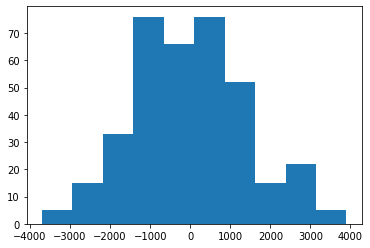
\includegraphics[scale=0.5]{callcenter.png}
    \caption{Статистика доходов колл центра за год}
\end{figure}

На гистограмме видно, что существует очень высокая вероятность потери прибыли. Давайте попробуем увеличить прибыль нашего колл центра не уменьшая зарплату работников. Например мы разработали алгоритм поиска потенциальных клиентов, благодаря этому увеличивается вероятность успешного звонка, а также, ориентируясь на конкретного клиента, мы уменьшаем время самого звонка.\\
В конечном итоге:
\begin{itemize}
  \item n = 53 звонков в день
  \item p = 4.5\%
\end{itemize}

\begin{figure}[h!]
    \centering
    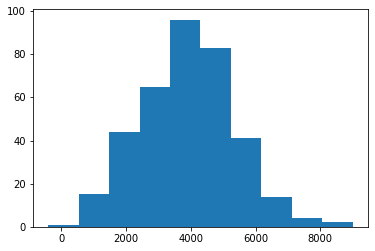
\includegraphics[scale=0.5]{callcenter2.png}
    \caption{Статистика доходов колл центра за год после внедрения алгоритма поиска потенциальных клиентов}
\end{figure}

Мы увеличили прибыль нашего колл центра! :)






\subsection{Нормальное распределение}

\subsubsection{Типичные интерпретации}

Если некая величина образуется в результате сложения многих случайных слабо взаимозависимых величин, каждая из которых вносит малый вклад относительно общей суммы, то центрированное и нормированное распределение такой величины при увеличении числа наблюдений стремится к нормальному распределению.

Это вытекает из центральной предельной теоремы теории вероятностей. Таких величин в окружающем нас мире очень много, поэтому такое распределение величин и названо нормальным. \\
Примеры:
\begin{itemize}
    \item Рост и вес человека;
    \item Ошибки наблюдений;
    \item Скорость молекул;
    \item Гауссовский процесс;
    \item Отклонение при стрельбе.
\end{itemize}

\section{Описание способа моделирования выбранных случайных величин}
Случайные величины для Биномиального и Нормального распределения можно смоделировать при помощи библиотеки NumPy из Python.\\

np.random.binomial(n, p, size) --- функция для моделирования случайных величин Биномиального распределения, где n --- это количество независимых случайных испытаний, p --- шанс успеха 
одного испытания, size --- объем выборки.\\
Пример использования: Посчитаем количество выпадения орлов для 10 бросков с объемом выборки $size=1000$

\begin{verbatim}

    np.random.binomial(n = 10, p = 0.5, size = 1000)

\end{verbatim}
\begin{figure}[h!]
    \centering
    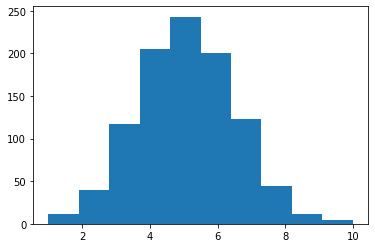
\includegraphics[scale=0.5]{example.png}
 
\end{figure}


np.random.normal($\mu$, $\sigma$, size) --- функция для моделирования случайных величин Нормального распределения, где $\mu$ и $\sigma$ --- это параметры нормального распределения математическое ожидание и среднеквадратичное отклонение соотвественно, , size --- объем выборки.\\
Пример использования:
\begin{verbatim}

    np.random.normal(mu = 0, sigma = 0.1, size = 1000)

\end{verbatim}

\begin{figure}[h!]
    \centering
    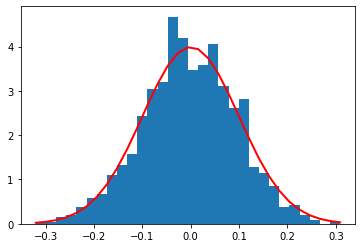
\includegraphics[scale=0.5]{example2.png}
 
\end{figure}

\bibliographystyle{unsrtnat}
\bibliography{references}

\end{document}
